\chapter{Réalisation, validation et mise en œuvre}

Ce dernier chapitre montre comment l'architecture présentée au chapitre précédent a été effectivement construite. Il présente l'environnement technique mobilisé, puis la réalisation des modules de la plateforme et de l'assistant conversationnel, avant de donner à voir cette réalisation du point de vue de l'utilisateur, à travers les interfaces et parcours réellement implémentés. Une campagne de validation confronte ensuite l'ensemble de ces réalisations à une exécution réelle, et un bilan referme ce chapitre en distinguant ce qui a été obtenu de ce qui reste, à ce stade, une limite assumée.

\section{Environnement technique}

\subsection{Environnement de calcul et de modélisation}

\begin{center}
\begin{tcbraster}[raster columns=3, raster equal height]
\techcard{figures/logos/python.svg}{Python}{Langage de programmation}{Environnement principal de développement et d'exécution des traitements de préparation des données, de modélisation du risque et des services métier.}
\techcard{figures/logos/git.svg}{Git}{Gestion de versions}{Suivi de l'évolution du code source, conservation de l'historique des modifications et organisation des changements apportés au projet.}
\techcard{figures/logos/github.svg}{GitHub}{Hébergement du dépôt}{Plateforme d'hébergement du dépôt Git du projet.}
\techcard{figures/logos/pandas.svg}{pandas}{Manipulation des données}{Nettoyage, transformation et préparation des jeux de données exploités par les moteurs de risque, présentés au chapitre 3.}
\techcard{figures/logos/scikitlearn.svg}{scikit-learn}{Apprentissage automatique}{Régression logistique, partitionnement K-means et outils de validation, utilisés pour la PD et la segmentation du portefeuille, chapitres 3 et 4.}
\techcardtext{XGBoost}{Apprentissage automatique}{Modèle de PD champion pour le segment Entreprises, et challenger pour le segment Particuliers, chapitre 3.}
\techcardtext{LightGBM}{Apprentissage automatique}{Modèle challenger de PD pour le segment Entreprises du suivi de portefeuille, et candidat évalué mais non retenu pour l'Origination, chapitre 3.}
\techcard{figures/logos/scipy.svg}{SciPy}{Calcul scientifique}{Optimisation numérique de la régression Beta utilisée pour la perte en cas de défaut, chapitre 3.}
\techcardtext{Optuna}{Optimisation d'hyperparamètres}{Recherche bayésienne des hyperparamètres des modèles XGBoost et LightGBM, par échantillonnage TPE, chapitre 3.}
\techcardtext{SHAP}{Interprétabilité}{Interprétabilité des modèles de PD par les valeurs de Shapley, présentée au chapitre 3.}
\techcardtext{joblib}{Sérialisation}{Sauvegarde et chargement des artefacts entraînés (modèles de PD, LGD, moteur de décision), chapitres 3 et 5.}
\end{tcbraster}
\end{center}

\subsection{Suivi des expérimentations}

\begin{center}
\begin{tcbraster}[raster columns=3, raster equal height]
\techcard{figures/logos/mlflow.svg}{MLflow}{Suivi d'expérimentation}{Suivi des runs d'entraînement du pipeline de modélisation présenté au chapitre 3 : paramètres, métriques et champion retenu par segment.}
\end{tcbraster}
\end{center}

\subsection{Environnement backend et accès aux données}

\begin{center}
\begin{tcbraster}[raster columns=3, raster equal height]
\techcard{figures/logos/fastapi.svg}{FastAPI}{Framework backend}{Expose les traitements de la plateforme sous forme d'API, consommée par l'application web présentée au chapitre 5.}
\techcard{figures/logos/sqlalchemy.svg}{SQLAlchemy}{Accès aux données}{Accès à la base PostgreSQL depuis le backend, notamment pour l'authentification et les services métier présentés au chapitre 5.}
\techcard{figures/logos/pydantic.svg}{Pydantic}{Validation des données}{Validation et structuration des données échangées par l'API, en particulier des requêtes d'évaluation de crédit.}
\techcard{figures/logos/jsonwebtokens.svg}{JWT}{Authentification}{Authentification des utilisateurs et gestion des jetons d'accès, selon les rôles présentés au chapitre 2.}
\end{tcbraster}
\end{center}

\subsection{Environnement de l'assistant conversationnel}

\begin{center}
\begin{tcbraster}[raster columns=3, raster equal height]
\techcard{figures/logos/pytorch.svg}{PyTorch}{Calcul tensoriel}{Exécution, en CPU, des modèles d'embeddings utilisés pour la recherche documentaire de l'assistant, chapitre 5.}
\techcardtext{sentence-transformers}{Embeddings}{Génération des embeddings sémantiques des passages documentaires, pour la recherche FAISS présentée au chapitre 5.}
\techcardtext{FAISS}{Recherche vectorielle}{Index de recherche sémantique local, combiné à une recherche lexicale, dans le mécanisme de recherche hybride de l'assistant, chapitre 5.}
\techcardtext{BM25}{Recherche lexicale}{Recherche lexicale, combinée à FAISS, dans le mécanisme de recherche hybride de l'assistant, chapitre 5.}
\techcardtext{pdfplumber}{Extraction documentaire}{Extraction du texte de la base documentaire réglementaire indexée par l'assistant, chapitre 5.}
\techcardtext{PyMuPDF}{Extraction documentaire}{Extraction principale du texte des documents soumis par un client ; un PDF scanné, sans texte extractible, bascule vers une reconnaissance optique.}
\techcard{figures/logos/paddlepaddle.svg}{PaddleOCR}{Reconnaissance optique}{Utilisée en repli uniquement, pour les documents scannés dont le texte n'est pas directement extractible par PyMuPDF.}
\techcard{figures/logos/langchain.svg}{LangChain}{Composants documentaires}{Composants de construction du pipeline d'extraction documentaire de l'assistant.}
\techcard{figures/logos/langgraph.svg}{LangGraph}{Orchestration}{Orchestration du graphe d'extraction documentaire des documents soumis lors d'une demande, présenté au chapitre 5.}
\techcardtext{Groq}{Génération de texte}{Fournisseur prioritaire de génération de texte pour l'assistant, présenté au chapitre 5.}
\techcard{figures/logos/anthropic.svg}{Anthropic}{Génération de texte}{Fournisseur alternatif de génération de texte, utilisé lorsque Groq n'est pas disponible, chapitre 5.}
\end{tcbraster}
\end{center}

\subsection{Environnement de test et de validation}

\begin{center}
\begin{tcbraster}[raster columns=3, raster equal height]
\techcard{figures/logos/pytest.svg}{pytest}{Tests automatisés}{Exécution des tests selon quatre marqueurs réels : unitaires, intégration base de données, chaînes de traitement et acceptation.}
\techcardtext{Playwright}{Tests d'acceptation}{Tests d'acceptation bout-en-bout des parcours Origination et Surveillance, en conditions de navigateur réel.}
\end{tcbraster}
\end{center}

Les résultats détaillés de ces tests, ainsi que les éventuelles anomalies identifiées, sont présentés en section~6.5.

\section{Réalisation des modules de la plateforme}

\subsection{Réalisation du parcours Origination}

Le parcours Origination, présenté aux chapitres 4 et 5, repose sur un service dédié à la gestion des dossiers, qui enregistre une demande puis déclenche son évaluation, et sur le service de crédit en ligne, point d'entrée unique du calcul métier déjà détaillé par le diagramme de séquence du chapitre 5. Ce dernier se déroule en deux étapes, la création du dossier puis son scoring, la seconde enchaînant une préparation des données, un calcul de Stage IFRS 9, puis sept sous-étapes internes au moteur de décision, de la vérification d'éligibilité jusqu'à l'explication SHAP, avant la persistance de la décision et, le cas échéant, l'ouverture d'un ticket de revue manuelle. Ces deux services sont exposés par un routeur dédié de l'API, et s'appuient sur un service de gouvernance des engagements distinct pour la gestion de la délégation présentée en section~4.5. Ces traitements mobilisent notamment un modèle de probabilité de défaut et un moteur de décision dédiés à l'Origination, présentés au chapitre 3, distincts de ceux utilisés pour le suivi de portefeuille. Les moteurs de perte en cas de défaut, d'exposition au défaut et de rentabilité reposent, quant à eux, sur les composants partagés entre les deux parcours, également présentés au chapitre 3.

\begin{figure}[H]
\centering
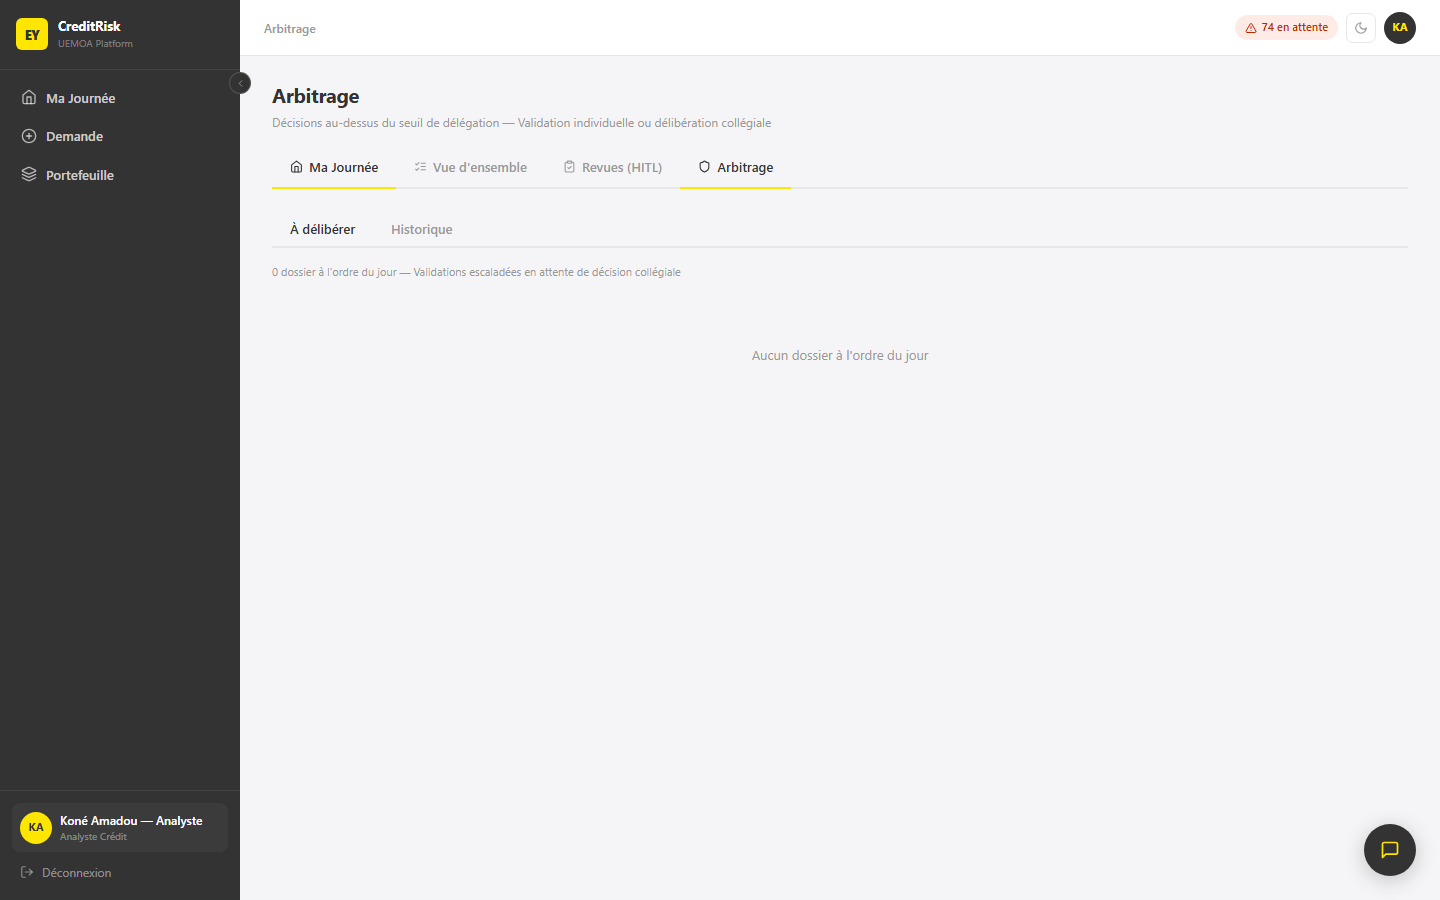
\includegraphics[width=0.85\textwidth]{figures/capture_delegation_arbitrage.png}
\caption{Écran d'arbitrage — décisions au-dessus du seuil de délégation, intégration réelle du service de gouvernance des engagements}
\label{fig:capture-delegation}
\end{figure}

La figure~\ref{fig:capture-delegation} illustre cette intégration : l'écran d'arbitrage, distinct de la file de revues manuelles présentée en section~4.5, n'affiche que les dossiers dont l'exposition dépasse le seuil de délégation de l'analyste connecté, et distingue explicitement la validation individuelle de la délibération collégiale.

\subsection{Réalisation du parcours Portfolio Analytics}

Le traitement batch du portefeuille, détaillé par le diagramme de séquence du chapitre 5, est réalisé par un orchestrateur unique qui enchaîne huit étapes déjà construites indépendamment, sans règle métier qui lui serait propre, de la construction de la population scorée jusqu'au calcul des signaux d'alerte précoce, avant une écriture finale dans l'ensemble des tables concernées au sein d'une unique transaction : toute exception survenant à n'importe quelle étape de cette écriture entraîne l'annulation complète de la transaction, de sorte qu'aucune table ne conserve un run partiellement enregistré. Les différents routeurs exposent les résultats de ce traitement batch pour le suivi général du portefeuille, les projections et les scénarios de stress, ainsi que l'analyse de la rentabilité. Ces traitements mobilisent les modèles entraînés destinés au suivi du portefeuille, présentés au chapitre 3, ainsi que les moteurs complémentaires présentés en section~4.4. Les modèles de probabilité de défaut utilisés dans ce parcours sont distincts de celui mobilisé lors de l'Origination.

\begin{figure}[H]
\centering
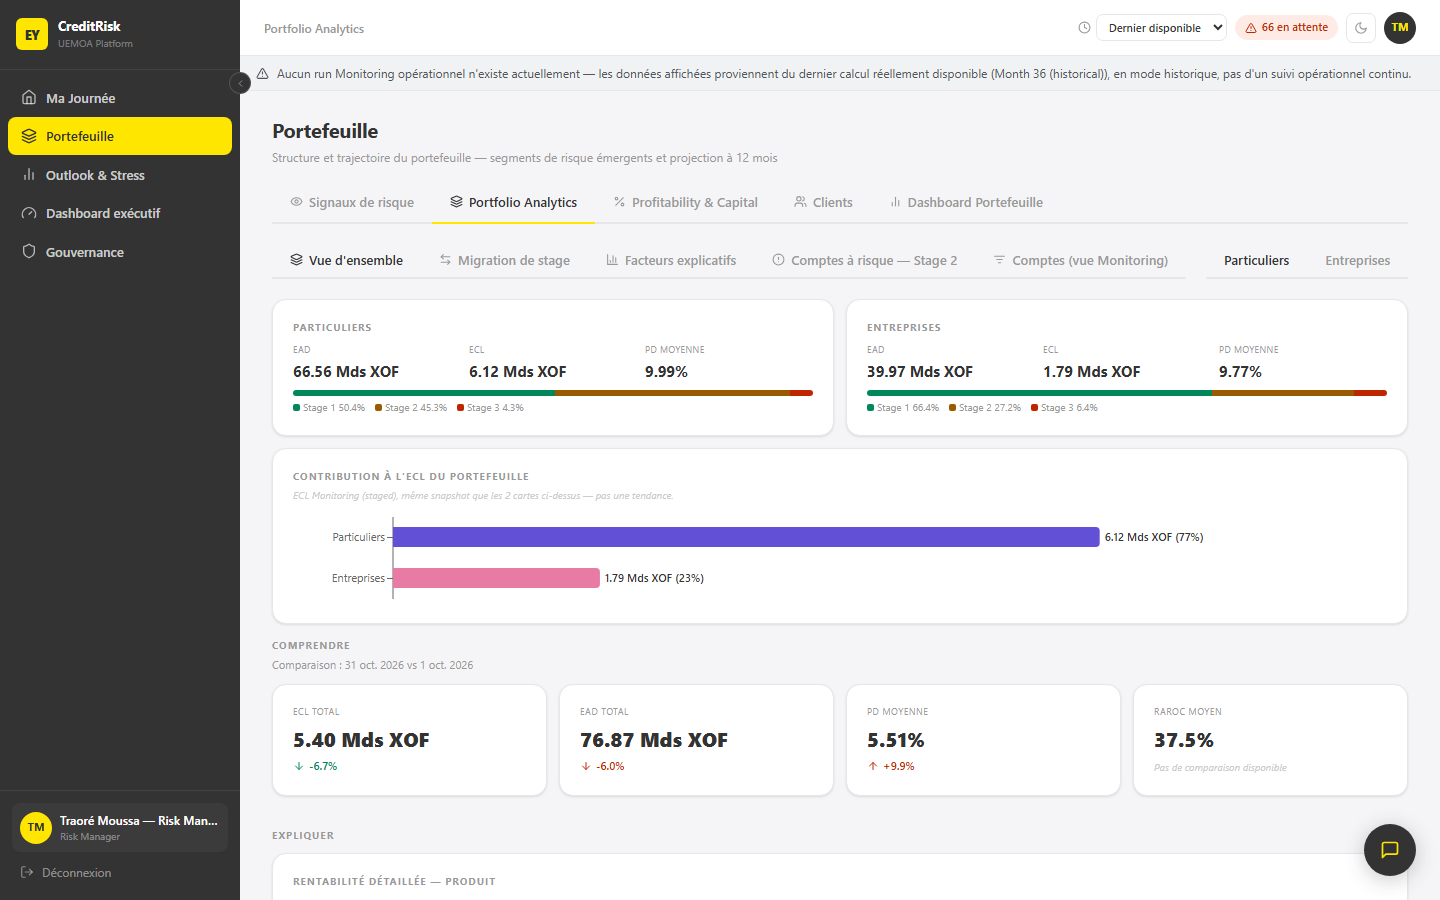
\includegraphics[width=0.85\textwidth]{figures/capture_portfolio_analytics.png}
\caption{Portfolio Analytics — résultats du traitement batch exposés par segment (Particuliers/Entreprises) et par Stage}
\label{fig:capture-portfolio-analytics}
\end{figure}

La figure~\ref{fig:capture-portfolio-analytics} donne à voir ce que recouvre concrètement « le suivi général du portefeuille » : l'exposition, l'ECL et la PD moyenne calculés par le batch, restitués par segment et par Stage, avec un bandeau de provenance qui rappelle explicitement que ces chiffres proviennent du dernier calcul réellement disponible plutôt que d'un suivi opérationnel continu, cohérent avec l'état réel du Monitoring déjà décrit au chapitre 4.

\subsection{Authentification et contrôle d'accès}

L'accès à la plateforme repose sur une authentification par jetons. La connexion d'un utilisateur produit un jeton d'accès de courte durée et un jeton de rafraîchissement, ce dernier conservé en base sous forme hachée plutôt qu'en clair. Le renouvellement d'un jeton d'accès fait tourner ce jeton de rafraîchissement : l'ancien est explicitement révoqué à chaque renouvellement, et la déconnexion révoque également le jeton en cours, de sorte qu'un jeton compromis ne reste pas valide indéfiniment.

Le contrôle d'accès par rôle, présenté au chapitre 2 pour les six rôles réels de la plateforme, chargé de clientèle, analyste crédit, Risk Manager, Direction, Conformité et Audit, Administrateur, n'est pas appliqué au seul niveau de l'interface : il est vérifié côté backend, par un mécanisme d'injection de dépendances propre à chaque point d'entrée de l'API. Ce mécanisme est effectivement mobilisé sur 91 points d'entrée répartis dans l'ensemble des routeurs de la plateforme, qu'il s'agisse de restreindre un endpoint à un rôle unique ou à un ensemble de rôles autorisés. Cette vérification s'exécute au niveau du point d'entrée de l'API lui-même, avant tout traitement métier : une tentative d'accès par un rôle non autorisé est donc rejetée indépendamment de l'interface cliente qui a émis la requête, qu'il s'agisse de l'application web présentée au chapitre 5 ou d'un appel direct à l'API.

\subsection{Traçabilité et gouvernance}

La traçabilité des traitements et des décisions, présentée au chapitre 2, repose sur un journal d'audit chaîné par hachage SHA-256, auquel s'ajoutent plusieurs tables de gouvernance. Les exécutions de la plateforme alimentent notamment les runs de pipeline, qu'ils soient d'entraînement, d'Origination en ligne ou de suivi de portefeuille, de même que les validations humaines requises par la délégation et les tickets de revue manuelle. À ces éléments produits par l'exécution s'ajoute la table des barèmes de délégation, qui relève à l'inverse de la configuration administrative plutôt que d'un événement d'exécution : elle conserve les seuils fixés pour encadrer les décisions, et non une trace de traitement. Cette gouvernance n'est donc pas qu'un mécanisme conçu, mais un ensemble de données réellement produites par les exécutions du projet, parmi lesquelles les runs déjà cités aux chapitres 4 et 5 pour illustrer le stress testing et le suivi de portefeuille.

\begin{figure}[H]
\centering
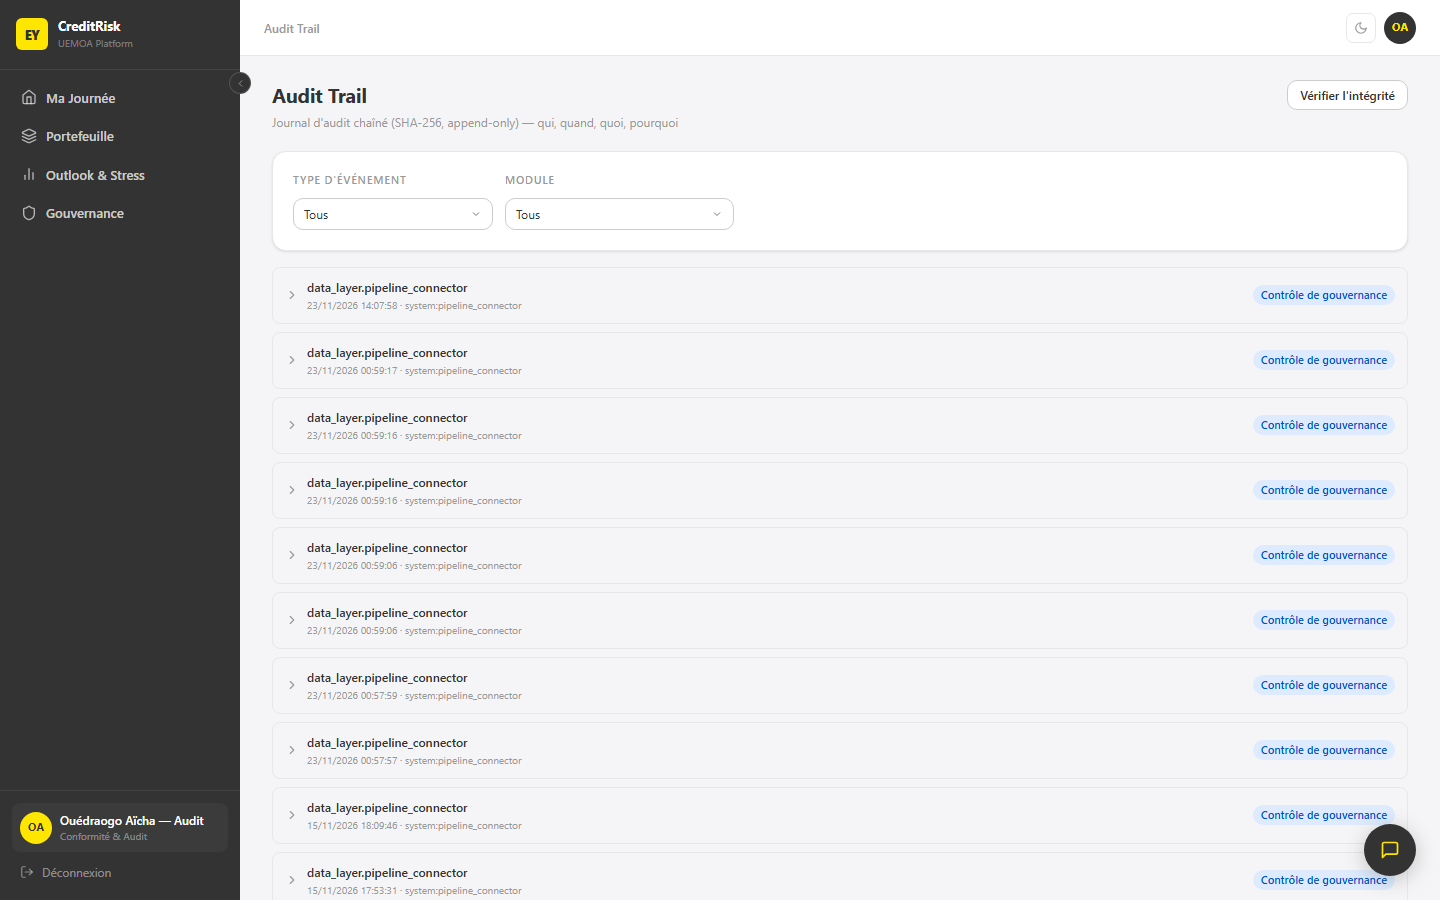
\includegraphics[width=0.85\textwidth]{figures/capture_audit_trail.png}
\caption{Journal d'audit chaîné — qui, quand, quoi, pourquoi, avec vérification d'intégrité}
\label{fig:capture-audit-trail}
\end{figure}

La figure~\ref{fig:capture-audit-trail} montre cette table telle qu'alimentée par l'exécution réelle de la plateforme, avec un bouton de vérification d'intégrité qui permet de contrôler, à tout instant, que la chaîne de hachage n'a pas été rompue.

Le barème de délégation mentionné au chapitre 4 comporte quatre paliers réels, administrés par un rôle Administrateur plutôt que codés en dur : pour le segment Particuliers, une décision reste automatique (AUTO) jusqu'à 5~millions de XOF d'exposition, requiert une validation individuelle (VALIDATION) jusqu'à 20~millions, et passe en comité de crédit (COMITE) au-delà ; pour le segment Entreprises, ces mêmes paliers s'échelonnent à 50~millions, 500~millions puis 2~milliards de XOF, un quatrième palier, le comité exécutif (COMITE\_EXECUTIF), s'appliquant au-delà de ce dernier montant. Ces plafonds sont des paramètres de politique de crédit propres au projet, et non une transposition de seuils réglementaires.

Le suivi du portefeuille mobilise par ailleurs deux autres familles de seuils, distinctes de la politique de décision. Quatre règles réelles déclenchent l'ouverture d'une revue de risque sur un compte déjà en portefeuille : le passage du Stage 1 au Stage 2 depuis l'origination, une hausse de la probabilité de défaut supérieure à 3~points depuis l'origination, un incident de paiement observé sur le dernier mois pour les Particuliers, et au moins deux dégradations de la notation depuis l'origination pour les Entreprises. La stabilité des modèles déployés est par ailleurs surveillée par un indice de stabilité de population (PSI). La plateforme retient les seuils conventionnels suivants pour l'interpréter : un indice inférieur à 0,10 signale une population stable, entre 0,10 et 0,25 une dérive modérée, et au-delà de 0,25 une dérive significative. Un contrôle de qualité des données, enfin, s'exécute en amont de chaque traitement batch, avec un seuil d'avertissement à 50~\% de valeurs manquantes sur une colonne, et un blocage strict en cas de doublons sur la clé naturelle d'une table ou de valeurs nulles sur une colonne clé.

\section{Réalisation de l'assistant intelligent}

\subsection{Intégration de l'assistant dans la plateforme}

Côté frontend, l'assistant n'est pas une page que l'utilisateur ouvrirait séparément : il est monté une seule fois, au niveau du conteneur applicatif (\texttt{AssistantProvider}, englobant \texttt{Layout} dans l'arborescence de composants), au-dessus du point où React Router substitue le contenu des pages. Le composant et son fournisseur restent ainsi montés lors de la navigation entre les écrans présentés en section~6.4 ; le changement de route ne provoque pas leur réinitialisation. Ce fournisseur expose un contexte global à deux niveaux : un contexte d'affichage léger, présenté dans le volet de l'assistant, et un contexte métier, transmis au backend pour contextualiser les requêtes, que chaque page met à jour à son entrée (page courante, type et identifiant de l'entité affichée le cas échéant). Le composant \texttt{FloatingAssistant}, superposé à toutes les pages via un bouton flottant, lit ce contexte pour adapter ses suggestions de questions au rôle de l'utilisateur connecté et à la page courante, et transmet l'identifiant d'entité de la page, lorsqu'il existe, à chaque question posée.

Cette architecture a une conséquence directe sur la résolution d'identité présentée au chapitre 5 : la contextualisation d'une question portant sur une entité affichée ne repose pas sur une résolution de référence à partir de l'historique conversationnel, mais sur l'identifiant de l'entité transmis par la page courante. Une question posée depuis la fiche d'un client porte donc implicitement sur ce client, sans que l'utilisateur ait besoin de le repréciser, tandis qu'une question posée depuis une page sans entité associée, par exemple le tableau de bord du portefeuille, ne porte sur aucun compte en particulier.

\subsection{Orchestration et traitement des requêtes}

Côté backend, un point d'entrée unique, \texttt{POST /api/assistant/ask}, reçoit la question ainsi que le contexte de page transmis par le frontend, puis délègue le traitement à \texttt{AIRiskAssistant.ask()}. Le déroulement complet de cette méthode, du contrôle des droits d'accès jusqu'à la double traçabilité, est représenté par le diagramme de séquence de la figure~\ref{fig:sequence-assistant} (section~5.5) ; cette sous-section présente les choix d'implémentation qui sous-tendent ce flux, sans en reprendre le détail pas à pas.

Le routeur met en œuvre les deux niveaux de classification présentés au chapitre 5 au moyen de mécanismes distincts : une détection par expressions régulières sur des mots-clés associés à chaque catégorie, dont le résultat est retenu dès que le seuil de confiance fixé à 0,70 est atteint, puis, seulement dans le cas contraire, un calcul de similarité cosinus entre l'embedding de la question et des exemples de référence par catégorie. Une question courte, de six mots ou moins, bénéficie en outre d'un mécanisme de contextualisation conversationnelle propre à ce routeur : lorsque la classification demeure incertaine, la catégorie de l'échange précédent est réutilisée plutôt que reclassée à vide. Ce mécanisme répond à une particularité du dialogue en langage naturel, absente des deux autres parcours de la plateforme : une question de relance, telle que « et pour les entreprises ? », ne porte souvent pas assez d'information pour être interprétée indépendamment du tour précédent.

La catégorie retenue est ensuite convertie en \textit{Scope} par une fonction dédiée. En l'absence de correspondance, celle-ci lève une exception plutôt que d'attribuer un périmètre par défaut. Cette vérification rend explicite toute catégorie non prise en charge et évite qu'elle soit traitée dans un périmètre inapproprié.

L'implémentation mutualise également une partie de ce traitement pour une seconde fonctionnalité, la génération d'un brief structuré de dossier client : contrairement à \texttt{ask()}, qui détermine la catégorie à partir de la question, \texttt{generate\_brief()} fixe directement la catégorie à CASE. Les deux méthodes s'appuient ensuite sur la même fonction interne, \texttt{\_answer\_from\_route()}, qui centralise le contrôle des droits, la validation des réponses, l'évaluation automatique et l'écriture en mémoire et dans les journaux d'audit, sans dupliquer ces mécanismes entre les deux usages ; seul l'historique conversationnel transmis au prompt diffère entre les deux, \texttt{generate\_brief()} ne le réutilisant pas, un brief de dossier étant par construction indépendant des échanges précédents.

\subsection{Recherche documentaire et système RAG}

Le moteur de recherche documentaire, déjà présenté au chapitre 5 pour son principe hybride FAISS/BM25, repose sur une boucle itérative de récupération et de vérification, pas une unique passe de recherche. À chaque itération, FAISS et BM25 sont interrogés indépendamment pour produire chacun une cinquantaine de passages candidats, dont l'union, plutôt qu'une fusion pondérée des deux scores, est ensuite reclassée par similarité cosinus entre l'embedding de la requête et celui de chaque passage candidat pour ne retenir que les \texttt{top\_k} passages finalement transmis au prompt. Si la réponse générée contient la mention explicite d'information non disponible, ou si son score de couverture sémantique, tel que nommé dans le code, reste sous un seuil fixé, le nombre de passages recherchés est doublé et une nouvelle itération est lancée, dans la limite de deux itérations de recherche au total par défaut, c'est-à-dire la recherche initiale suivie d'au plus une relance, ce seuil comme le nombre d'itérations maximal restant paramétrables par variable d'environnement. Ce score mesure une similarité cosinus entre le contexte retourné et la réponse produite. Il s'agit d'un indicateur de proximité sémantique, et non d'une vérification factuelle garantissant que chaque élément de la réponse est effectivement justifié par les documents retrouvés. Cette base documentaire étant majoritairement rédigée en anglais, la requête de recherche, mais non la question posée à l'utilisateur, est enrichie de termes anglais équivalents lorsqu'elle contient une expression courante du vocabulaire IFRS 9 en français, afin d'améliorer le rappel sans altérer la question reformulée dans la réponse.

Le contexte documentaire retrouvé, de même que l'historique conversationnel et le contexte de page transmis par le frontend, sont délimités explicitement dans le prompt avant d'y être insérés, jamais traités comme une instruction système, selon deux catégories distinctes définies dans le code : le contexte documentaire, qui ne provient pas du client mais d'une base indexée, et l'historique conversationnel ainsi que le contexte de page, effectivement fournis par le client à chaque requête. Les sources restituées à l'utilisateur, au format « [document - page] », sont extraites par reconnaissance de motif directement depuis le contexte documentaire retrouvé, et non depuis le texte de la réponse générée par le modèle : l'extraction porte sur ce qui a effectivement été récupéré par la recherche hybride, pas sur ce que le modèle a choisi de citer, ce qui limite l'affichage de références absentes du contexte effectivement récupéré, sans garantir pour autant que chaque passage récupéré ait été utilisé dans la réponse elle-même.

\subsection{Génération des réponses et mécanismes de repli}

La génération du texte de réponse repose sur une interface commune, implémentée par deux fournisseurs de génération externes et un fournisseur déterministe de dernier recours, plutôt que sur un modèle unique figé dans le code. Au démarrage de l'assistant, une fonction dédiée retient le premier fournisseur effectivement disponible parmi les trois, dans un ordre fixe : Groq, s'il expose une clé d'API valide et parvient à initialiser son client ; Anthropic sinon, selon le même principe ; le fournisseur déterministe en dernier recours, qui ne dépend d'aucun service externe et reste donc toujours disponible. Cette disponibilité est vérifiée une seule fois, à la construction de l'assistant, et non à chaque question : un fournisseur qui deviendrait indisponible en cours d'exécution, après ce choix initial, ne déclenche pas de bascule automatique vers le suivant.

Le fournisseur de dernier recours ne doit pas être confondu avec un troisième modèle génératif : il ne produit aucun texte original, mais retourne l'une de quelques réponses préécrites, sélectionnée par une simple détection de mots-clés dans la question (Stage 2, ECL, RAROC, motif de rejet). Son rôle n'est pas de répondre correctement à une question arbitraire, mais de fournir une réponse de secours lorsqu'aucun fournisseur de génération externe n'est disponible à l'initialisation, notamment lors d'un développement local sans clé d'API. Cette distinction a une conséquence directe sur l'interprétation d'une réponse de l'assistant au moment des tests ou d'une démonstration : les réponses de ce fournisseur de dernier recours sont fixes pour un même mot-clé détecté, quelle que soit la formulation exacte de la question ou le fil de la conversation, un indice observable que l'assistant fonctionne en mode de repli plutôt qu'avec un fournisseur de génération réel.

\subsection{Sécurité et traçabilité}

Le filtrage RBAC déjà présenté au chapitre 5 est implémenté selon un principe de refus par défaut (\textit{fail-closed}), plutôt que sous la forme d'une liste de restrictions ajoutées au cas par cas : un rôle absent de la table des périmètres autorisés ne se voit attribuer aucune catégorie de donnée sensible. Cette approche évite notamment qu'un périmètre vide soit interprété comme une autorisation illimitée à la suite d'une erreur de configuration. Chaque résultat de requête est filtré récursivement, champ par champ, les catégories étant déterminées à partir de conventions de nommage déjà utilisées dans les moteurs spécialisés (un champ contenant \texttt{shap} ou \texttt{raroc}, par exemple, relève respectivement de l'interprétabilité ou de la rentabilité). Un conteneur dont tous les champs ont été supprimés après filtrage est lui-même retiré du résultat, plutôt que conservé sous la forme d'un objet vide, afin de ne pas exposer indirectement la structure de données non autorisées.

Une fois la réponse assemblée, une seconde couche, distincte du filtrage RBAC, vérifie sa cohérence avant qu'elle n'atteigne l'utilisateur. Cette couche de validation effectue quatre contrôles successifs, chacun pouvant à lui seul entraîner le rejet de la réponse entière : l'ancrage, qui rejette une réponse lorsque des faits vérifiables sont disponibles mais qu'aucun n'est cité ; la validité des références, qui doivent toutes correspondre à un fait effectivement fourni au modèle ; la provenance, chaque fait cité étant revérifié à partir de son artefact source exact ; et la cohérence avec l'écran, pour les faits disposant d'une méthode de vérification dédiée, la valeur citée étant comparée à celle réellement affichée par l'interface. Cette couche ne garantit pas l'exactitude de toute réponse produite. Elle réduit le risque qu'un fait explicitement vérifiable soit présenté alors que sa validité n'est plus confirmée par sa source. Elle ne garantit toutefois pas l'exactitude de l'ensemble du texte formulé librement par le modèle autour de ces faits.

Une évaluation automatique complémentaire est également réalisée, sans se substituer à cette validation : elle combine des métriques de similarité entre les embeddings du contexte et de la réponse avec un jugement produit par un second appel au modèle de langage, selon des critères de correction, de fidélité, d'absence d'hallucination et de pertinence métier. Cette évaluation repose donc elle-même sur un modèle de langage chargé de juger la réponse d'un autre modèle. Son résultat est journalisé à titre d'indicateur de suivi et n'intervient pas dans la décision de rejeter ou non la réponse, déjà prise par la couche de validation précédente.

Enfin, chaque interaction fait l'objet de deux enregistrements indépendants : une entrée dans le journal dédié à l'assistant, propre à ce sous-système, et une entrée dans le journal d'audit central de la plateforme, présenté au chapitre 2. La seconde écriture est conçue pour être non bloquante : un échec de l'enregistrement dans le journal d'audit central est intercepté et ne doit pas interrompre le traitement de la réponse. Ainsi, une indisponibilité de ce mécanisme de traçabilité ne bloque pas, à elle seule, la restitution d'une réponse déjà produite et validée.

\section{Interface et parcours utilisateurs}

Alors que la section 6.2 démontrait, par quelques captures ciblées, l'intégration technique des modules décrits au chapitre 5, cette section présente l'ensemble des interfaces fonctionnelles réellement accessibles, organisées non par module technique mais par parcours utilisateur. La structure retenue suit l'arborescence de navigation réellement implémentée (\texttt{App.jsx}, \texttt{navigation.js}) plutôt qu'un découpage reconstruit a posteriori : six destinations de premier niveau, accessibles depuis la barre latérale selon le rôle de l'utilisateur connecté, auxquelles s'ajoutent l'écran de connexion et l'assistant conversationnel, ce dernier n'étant pas une destination de navigation mais un composant flottant superposé à l'ensemble de ces écrans. Chaque parcours est présenté sous la forme d'une courte user story, acteur, objectif, interaction et résultat, illustrée par une capture d'écran réelle ; les rôles mentionnés sont strictement ceux effectivement autorisés par le contrôle d'accès présenté en section~6.2.3, aucun acteur ni aucune permission n'étant ici supposés.

\subsection{Accès à la plateforme}

\begin{description}
\item[Acteur] Tout utilisateur détenteur d'un compte, quel que soit son rôle.
\item[Objectif] Accéder à son espace de travail.
\item[Interaction] Saisie de l'identifiant et du mot de passe, puis authentification par jeton présentée en section~6.2.3.
\item[Résultat] Redirection vers l'espace « Ma Journée », dont le contenu dépend du rôle authentifié.
\end{description}

\begin{figure}[H]
\centering
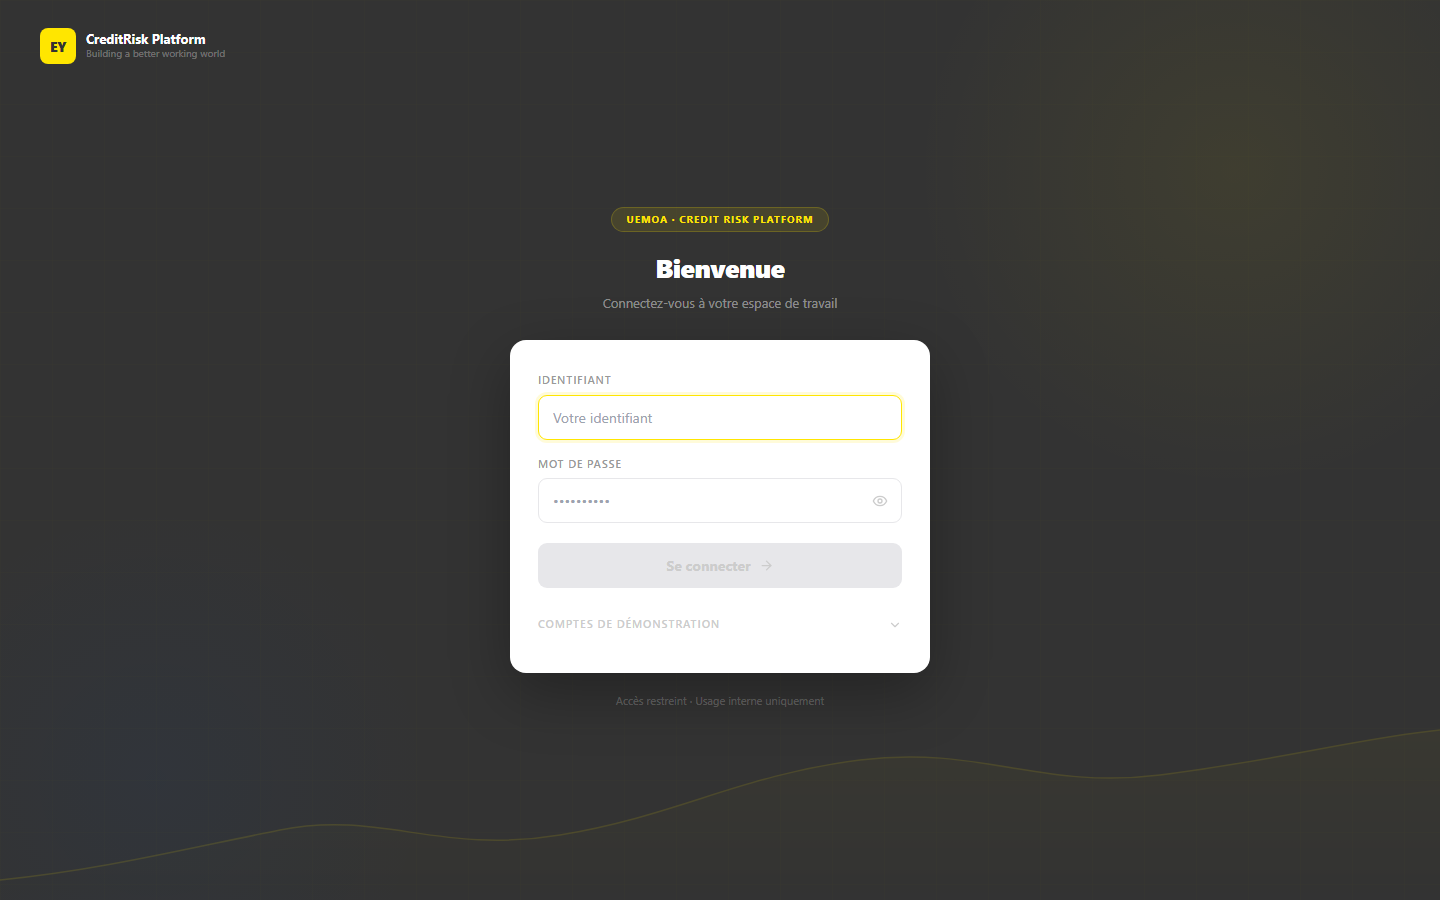
\includegraphics[width=0.6\textwidth]{figures/capture_login.png}
\caption{Écran de connexion}
\label{fig:capture-login}
\end{figure}

\subsection{Ma Journée}

\begin{description}
\item[Acteur] Analyste crédit ou Risk Manager.
\item[Objectif] Suivre les dossiers à traiter dans la journée : revues manuelles en zone grise, et, le cas échéant, dossiers à arbitrer au-delà du seuil de délégation.
\item[Interaction] Consultation de la vue d'ensemble, qui agrège sept sources de travail actionnable, puis ouverture de l'onglet « Revues (HITL) » pour traiter une décision en zone grise nécessitant un arbitrage humain.
\item[Résultat] La liste des revues en attente, filtrable par statut et par segment, permet à l'analyste de sélectionner un dossier et de rendre sa décision.
\end{description}

\begin{figure}[H]
\centering
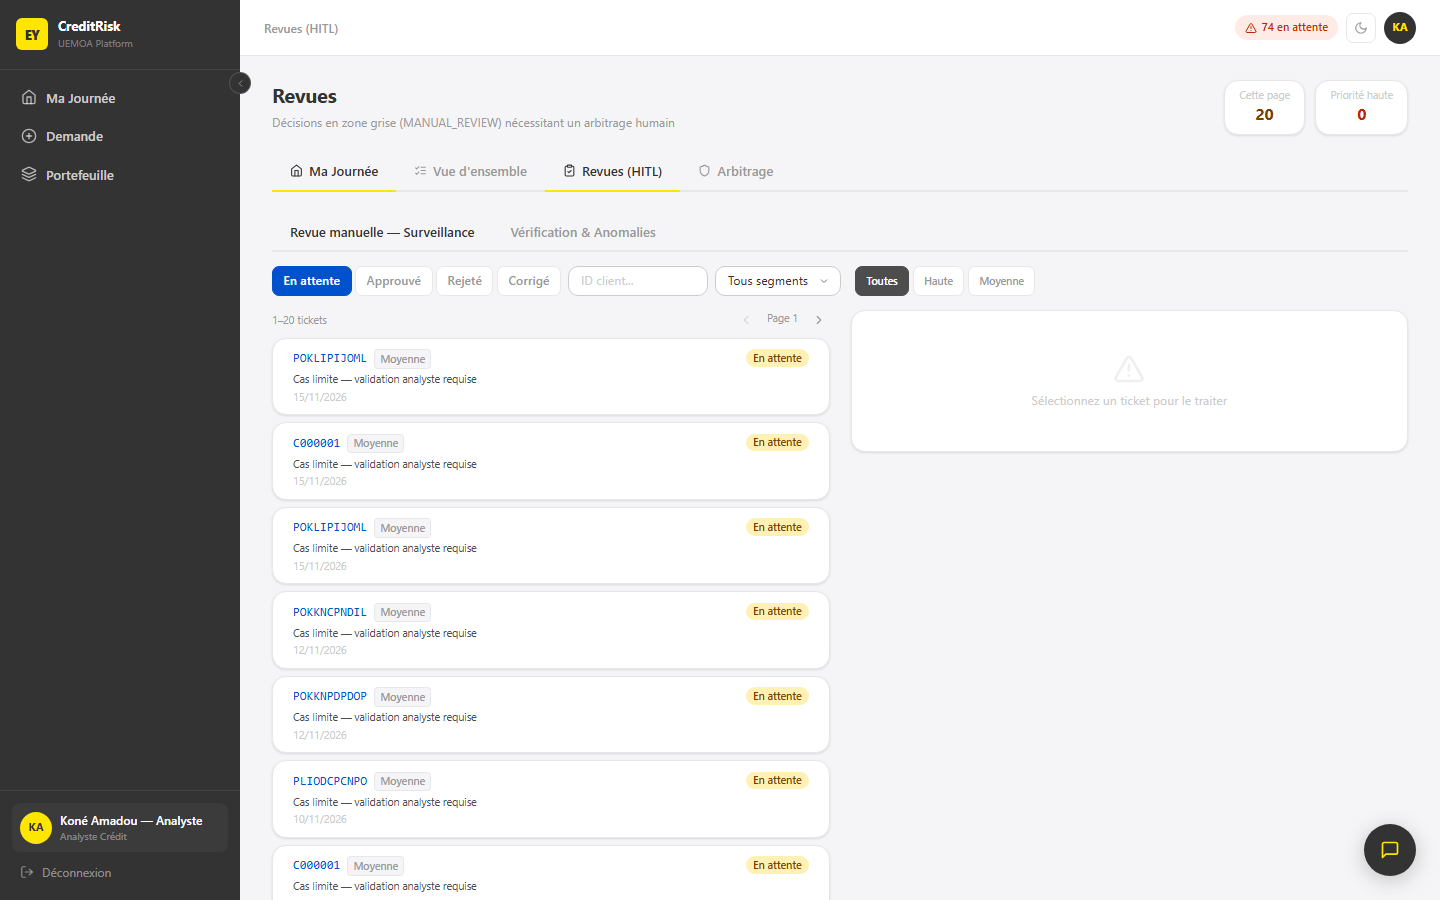
\includegraphics[width=0.85\textwidth]{figures/capture_hitl.png}
\caption{Ma Journée — Revues (HITL), décisions en zone grise nécessitant un arbitrage humain}
\label{fig:capture-hitl}
\end{figure}

\subsection{Demande}

\begin{description}
\item[Acteur] Chargé de clientèle (analyste crédit également habilité).
\item[Objectif] Créer une nouvelle demande de crédit pour un client existant, puis suivre les dossiers déjà engagés.
\item[Interaction] Sélection du client, puis progression dans un parcours en six étapes, demande, situation, risque de la demande, décision, explication et action, avant de retrouver le dossier dans la liste « Dossiers ». Dès la première étape, le chargé de clientèle peut transmettre un document du client, bulletin de salaire, relevé bancaire ou bilan selon le segment ; une extraction réelle, à partir du texte directement extrait du document ou, pour un document scanné sans texte extractible, d'une reconnaissance optique de repli, puis structurée par un modèle de langage, en déduit automatiquement plusieurs champs du formulaire, chacun assorti d'un niveau de confiance, les champs dont la confiance reste sous un seuil de 0,75 étant explicitement signalés et devant être confirmés ou corrigés avant de poursuivre. La dernière étape diffère selon l'issue remappée à l'écran, accord, refus ou à revoir : un accord sous conditions y ouvre un panneau de résolution des conditions, soumis à une permission dédiée, tandis qu'un refus ou un dossier à revoir donne accès, lorsqu'elle est disponible, à l'explication contrefactuelle déjà produite par le moteur, ainsi qu'à un simulateur \textit{What-If} réel permettant d'évaluer l'effet d'un paramètre modifié sur le résultat, sans modifier le dossier initial ni remplacer sa décision enregistrée.
\item[Résultat] Chaque dossier conserve son statut, complet, à revoir ou clôturé, avec son issue, accord, refus ou à revoir, et le montant associé.
\end{description}

\begin{figure}[H]
\centering
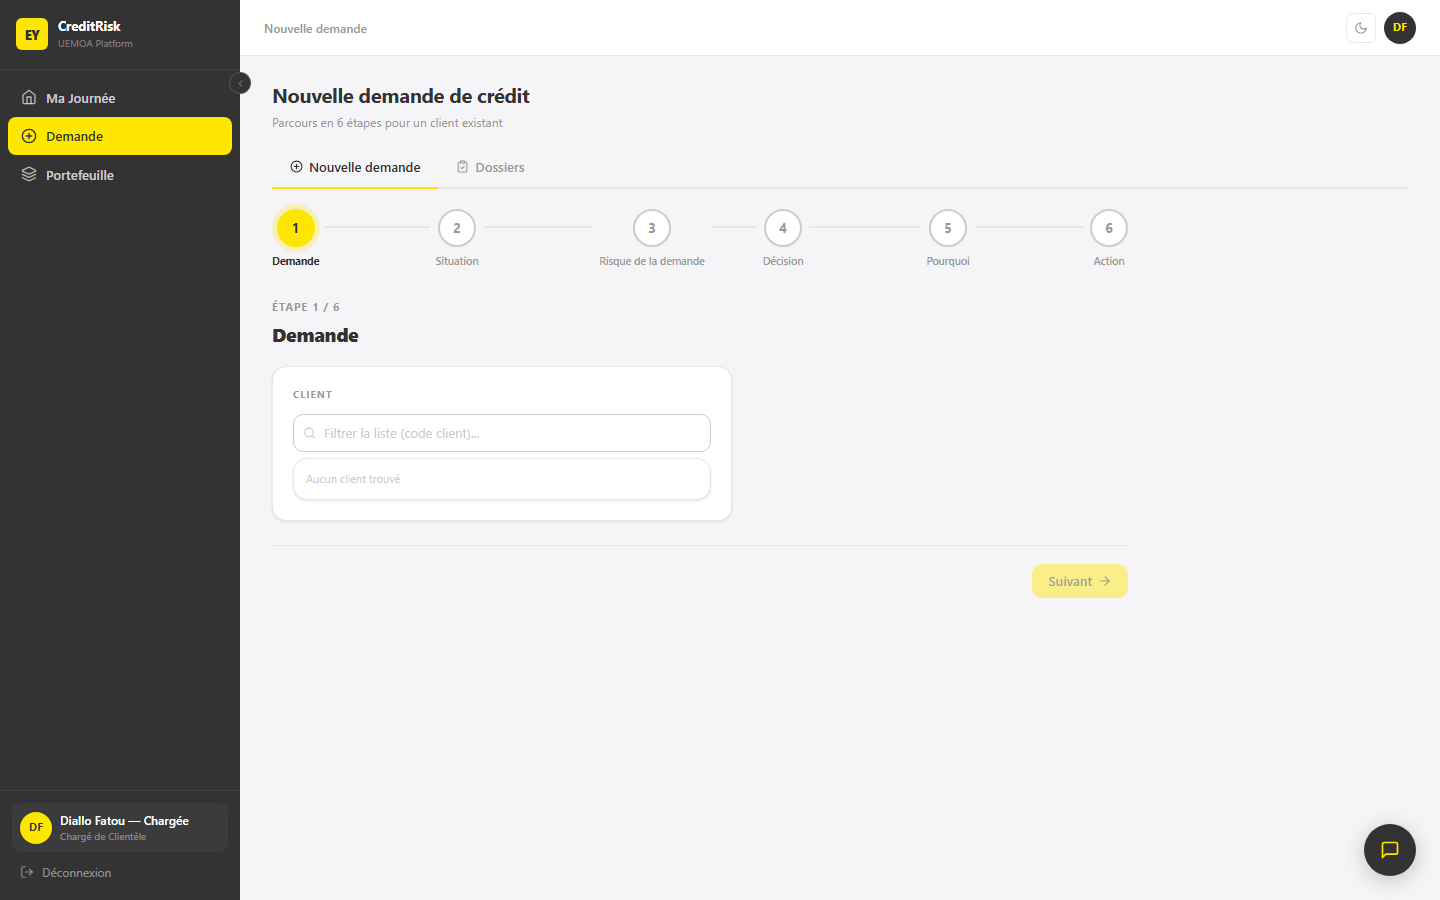
\includegraphics[width=0.85\textwidth]{figures/capture_demande_nouvelle.png}
\caption{Demande — parcours en six étapes de création d'une demande de crédit}
\label{fig:capture-demande-nouvelle}
\end{figure}

\begin{figure}[H]
\centering
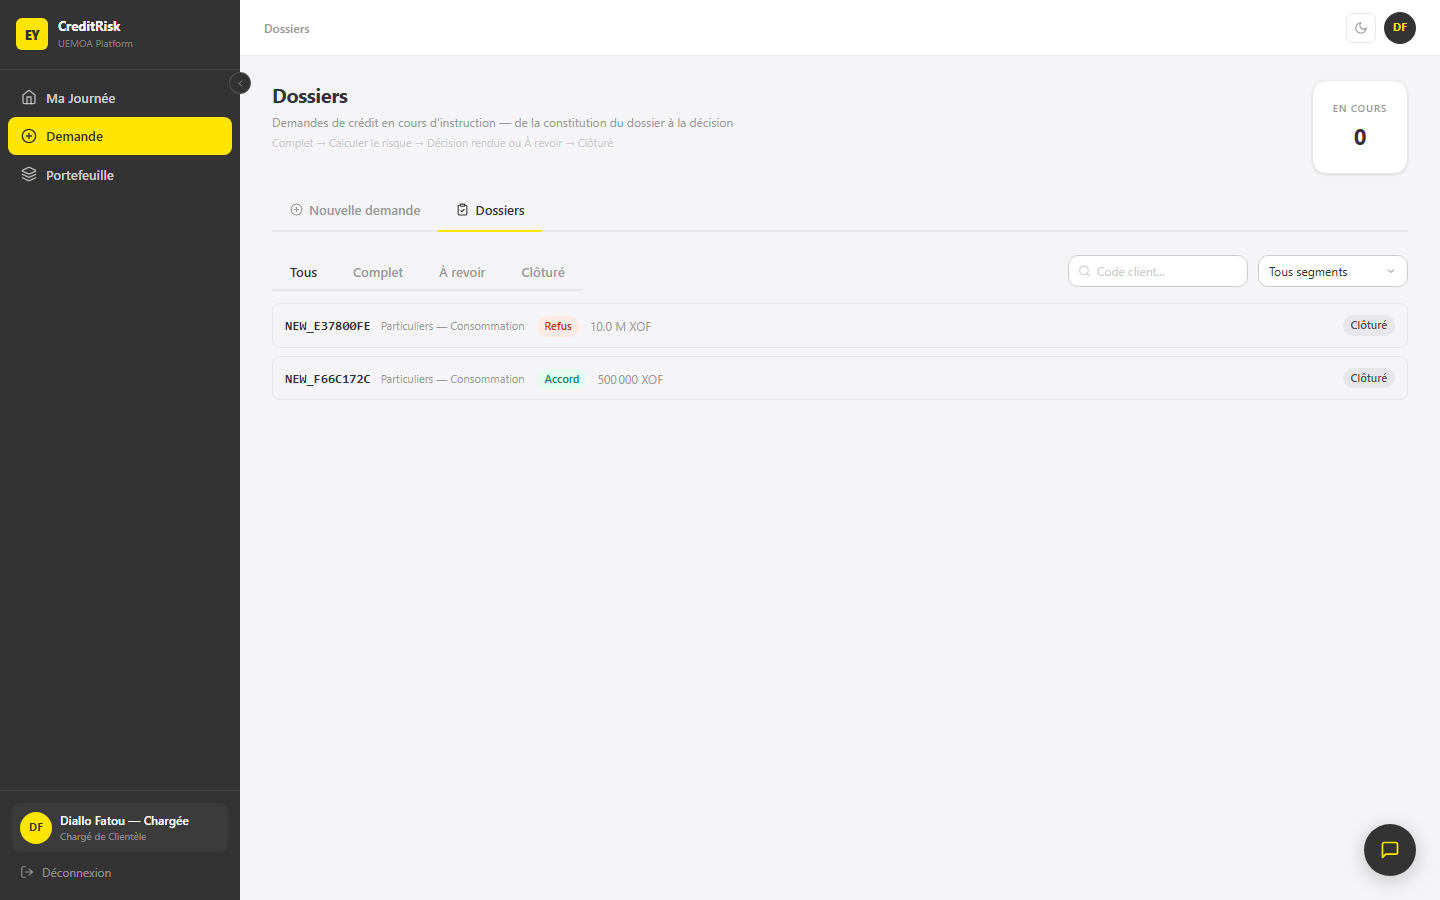
\includegraphics[width=0.85\textwidth]{figures/capture_demande_dossiers.png}
\caption{Demande — suivi des dossiers, de leur instruction à leur décision}
\label{fig:capture-demande-dossiers}
\end{figure}

\subsection{Portefeuille}

\begin{description}
\item[Acteur] Risk Manager, dont le périmètre couvre l'ensemble des cinq onglets de cette destination (l'Exécutif et l'analyste crédit n'y accèdent que partiellement).
\item[Objectif] Explorer la composition et la trajectoire du portefeuille : signaux de risque, analyse détaillée par segment et par Stage, rentabilité et capital, fiche Client 360°.
\item[Interaction] Consultation du tableau de bord Portefeuille, synthèse native du traitement batch présenté en section~6.2.2, puis navigation vers les onglets de détail selon le besoin.
\item[Résultat] Une vue de la composition du portefeuille par segment et par Stage, avec sa tendance par rapport au run précédent, et un bandeau de provenance rappelant explicitement l'origine des données affichées.
\end{description}

\begin{figure}[H]
\centering
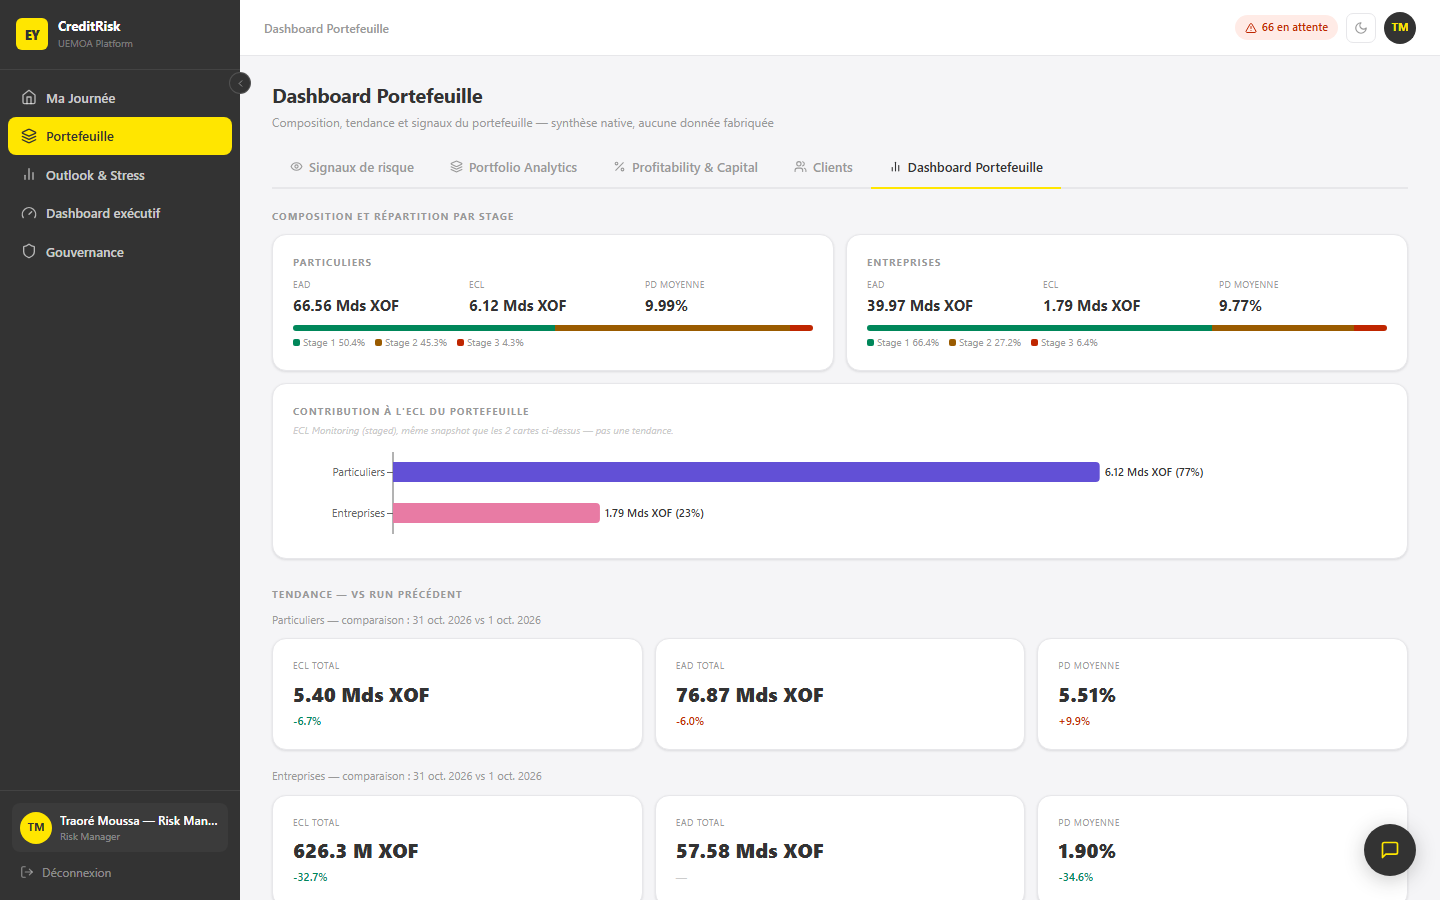
\includegraphics[width=0.85\textwidth]{figures/capture_portfolio_dashboard.png}
\caption{Portefeuille — tableau de bord natif, composition et tendance par rapport au run précédent}
\label{fig:capture-portfolio-dashboard}
\end{figure}

\subsection{Outlook \& Stress}

\begin{description}
\item[Acteur] Risk Manager (Exécutif et Conformité également habilités).
\item[Objectif] Examiner l'évolution projetée du portefeuille et sa résistance à des chocs macroéconomiques hypothétiques, présentées en section~4.4.
\item[Interaction] Consultation de l'onglet Outlook, qui restitue la projection à douze mois glissants par Stage IFRS9 avec sa bande d'incertitude P5/P50/P95, avant de basculer, au besoin, vers les onglets Stress Testing ou Capital \& Policy Simulation.
\item[Résultat] Une trajectoire indicative assortie d'avertissements méthodologiques explicites : la projection n'est pas un engagement chiffré, et la bande d'incertitude statistique ne doit pas être confondue avec l'impact d'un scénario de stress macroéconomique.
\end{description}

\begin{figure}[H]
\centering
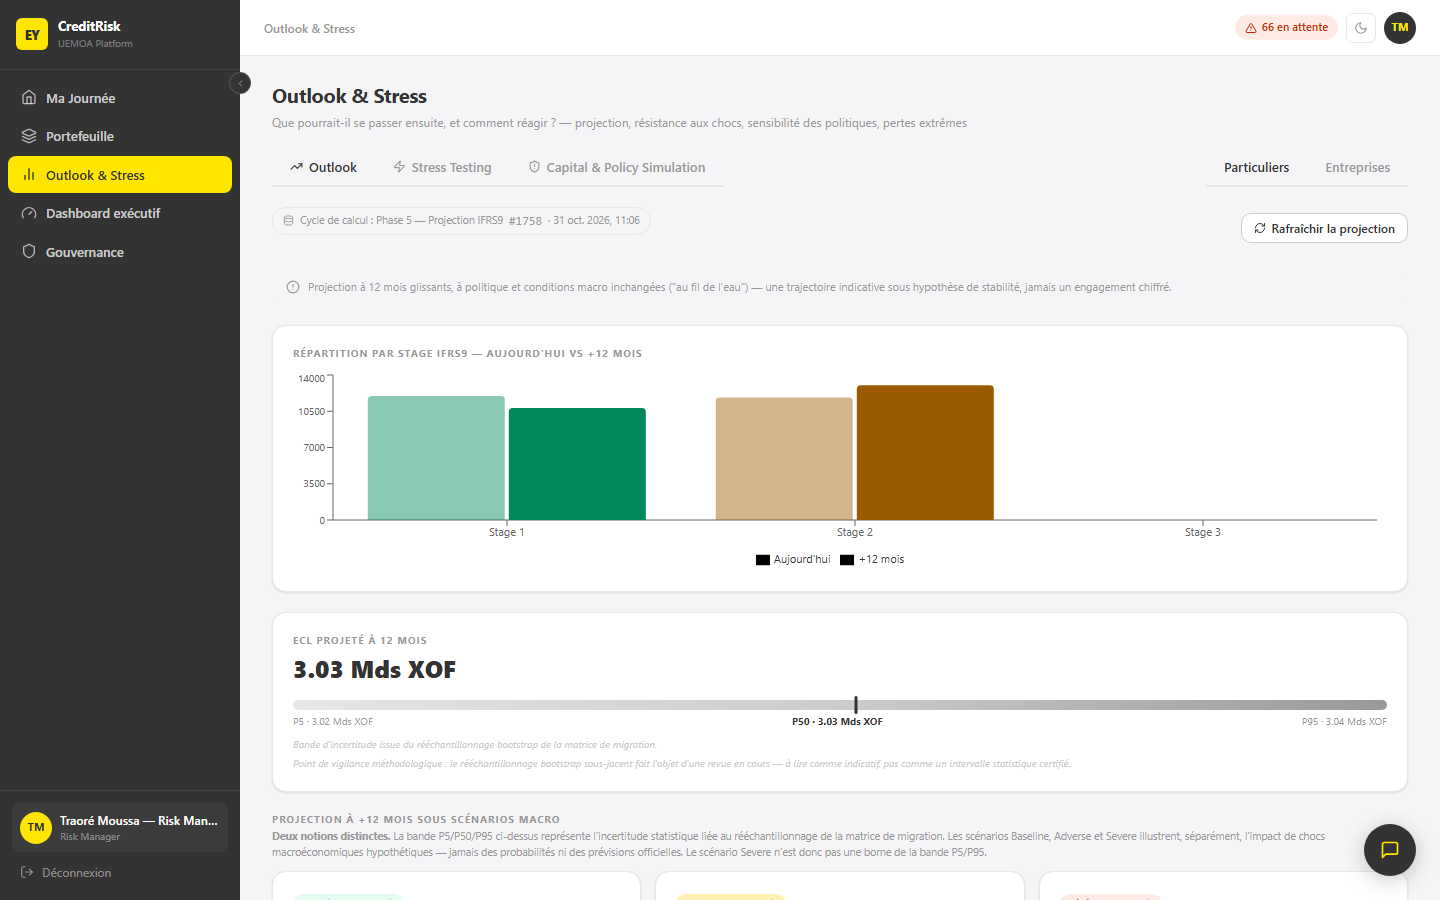
\includegraphics[width=0.85\textwidth]{figures/capture_outlook_stress.png}
\caption{Outlook \& Stress — projection à 12 mois par Stage IFRS9, avec bande d'incertitude et avertissements méthodologiques}
\label{fig:capture-outlook-stress}
\end{figure}

\subsection{Dashboard exécutif}

\begin{description}
\item[Acteur] Direction (Risk Manager également habilité).
\item[Objectif] Disposer d'une synthèse transversale pour le pilotage de l'activité, sans capacité opérationnelle.
\item[Interaction] Consultation du dashboard exécutif, qui agrège en lecture seule les indicateurs déjà présentés dans les autres destinations, exposition, pertes attendues, capital, rentabilité et résultats des stress tests, sans dupliquer leur calcul.
\item[Résultat] Une vue consolidée qui rend explicites, plutôt que de les masquer, les limites méthodologiques déjà rencontrées au chapitre 4 : les deux bases de capital, proxy réglementaire et Monte Carlo, restent présentées séparément et jamais sommées, et le RAROC agrégé au niveau du portefeuille est signalé comme non consolidé faute de convention d'agrégation unique entre les différents pipelines.
\end{description}

\begin{figure}[H]
\centering
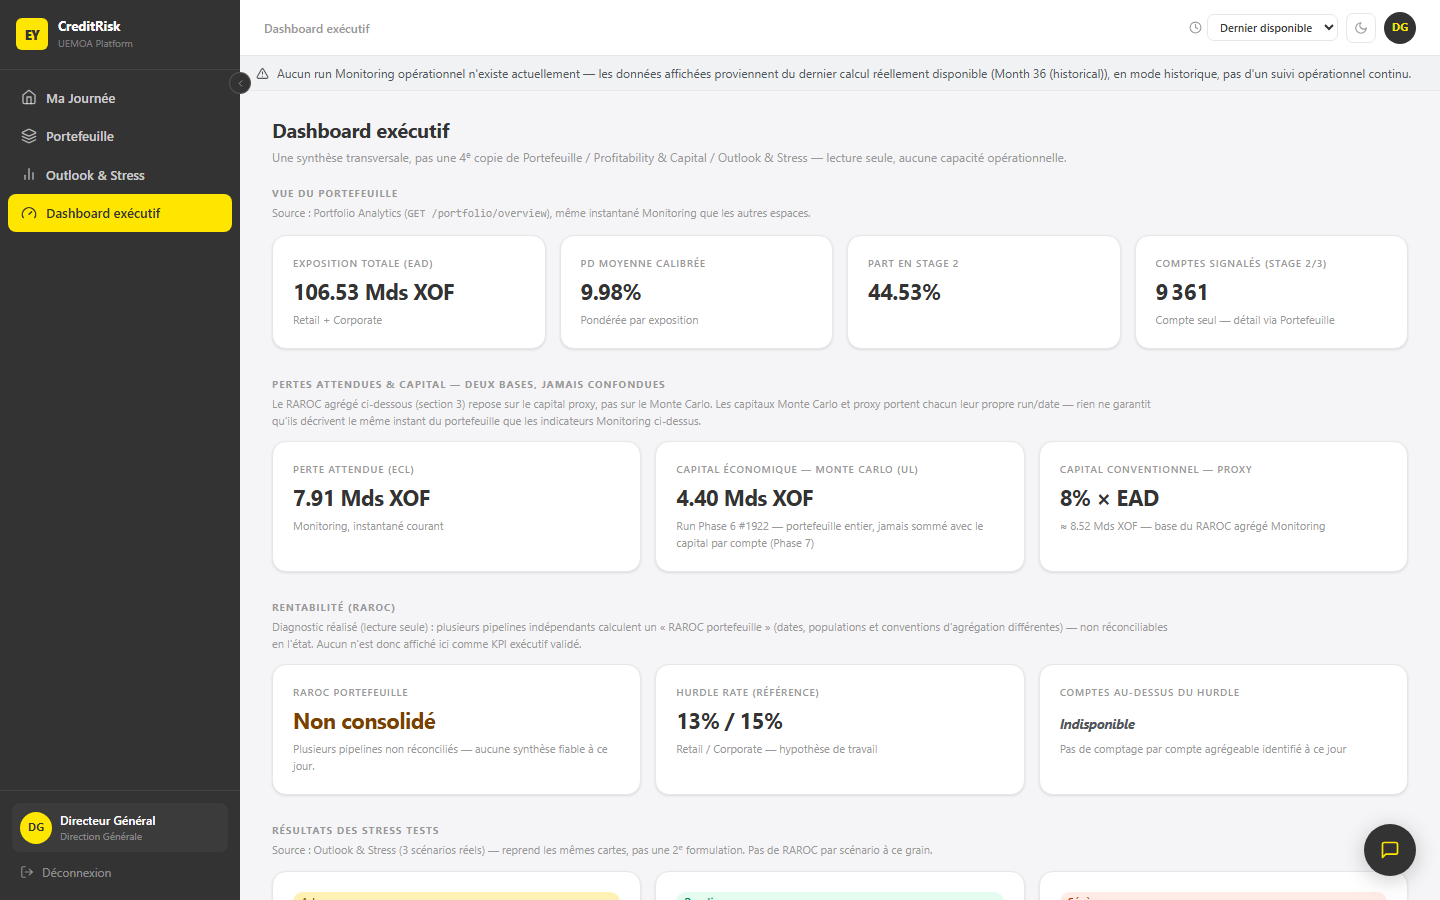
\includegraphics[width=0.85\textwidth]{figures/capture_dashboard_executif.png}
\caption{Dashboard exécutif — synthèse transversale en lecture seule, capital proxy et Monte Carlo jamais confondus}
\label{fig:capture-dashboard-executif}
\end{figure}

\subsection{Gouvernance}

\begin{description}
\item[Acteur] Conformité et Audit pour l'audit trail, la politique de décision, l'inventaire des modèles et les traitements batch ; Administrateur, seul habilité, pour les seuils de délégation et la gestion des utilisateurs et rôles ; Risk Manager pour les Trigger Rules.
\item[Objectif] Consulter, et selon son rôle administrer, les mécanismes de contrôle de la plateforme.
\item[Interaction] Ouverture du hub Gouvernance, dont les sept cartes renvoient chacune vers l'écran réel correspondant avec le même contrôle d'accès que la navigation : une carte à laquelle l'utilisateur connecté n'est pas habilité apparaît grisée, verrouillée et explicitement annotée « Non accessible à votre rôle », plutôt que d'être simplement absente.
\item[Résultat] Pour un compte Conformité et Audit, quatre cartes sur sept sont accessibles, audit trail, politique de décision, modèles, traitements batch, les trois autres restant verrouillées, ce qui illustre concrètement que ce hub ne correspond pas à un acteur unique mais à plusieurs périmètres de rôle distincts. Les cartes Seuils de délégation et Trigger Rules donnent accès aux paramètres déjà présentés en section~6.2.4.
\end{description}

\begin{figure}[H]
\centering
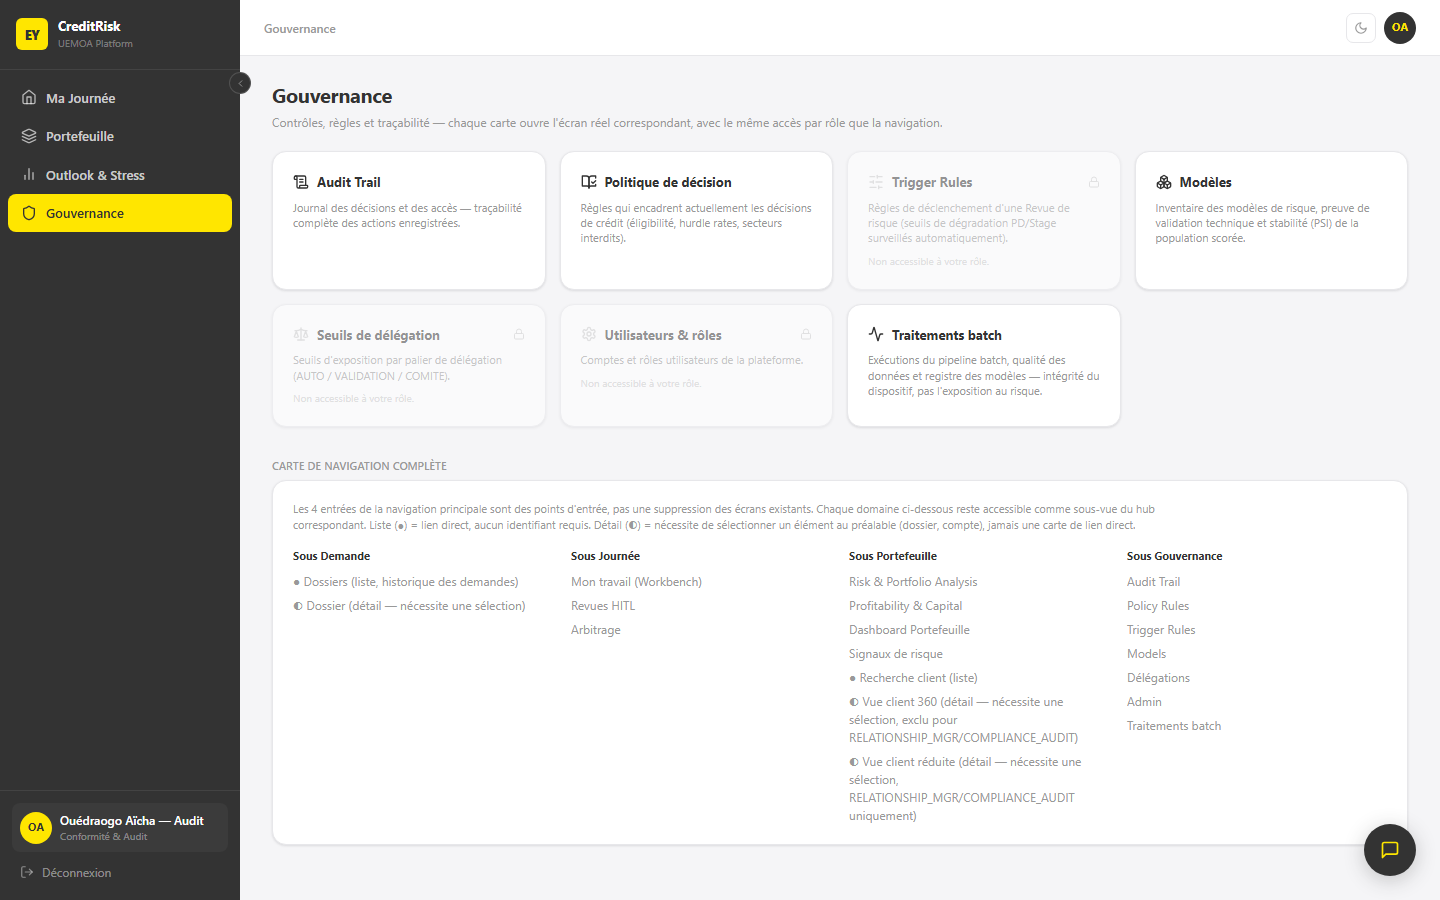
\includegraphics[width=0.85\textwidth]{figures/capture_gouvernance_hub.png}
\caption{Hub Gouvernance — sept cartes, contrôle d'accès visible par carte (vue Conformité et Audit)}
\label{fig:capture-gouvernance-hub}
\end{figure}

\subsection{Assistant transversal}

\begin{description}
\item[Acteur] Tout utilisateur authentifié.
\item[Objectif] Obtenir, depuis n'importe quel écran, une réponse contextualisée sans interrompre son parcours.
\item[Interaction] Ouverture du composant flottant, visible en superposition sur l'ensemble des écrans précédents, puis formulation d'une question en langage naturel.
\item[Résultat] Une réponse contextualisée, qui peut s'appuyer sur la base documentaire réglementaire présentée au chapitre 5 et restituer les références documentaires correspondantes lorsqu'elles sont disponibles, ou sur les moteurs métier du portefeuille et des dossiers clients selon la nature de la question ; lorsque les éléments accessibles ne permettent pas de répondre précisément, l'assistant le signale plutôt que de produire une réponse non étayée.
\end{description}

\begin{figure}[H]
\centering
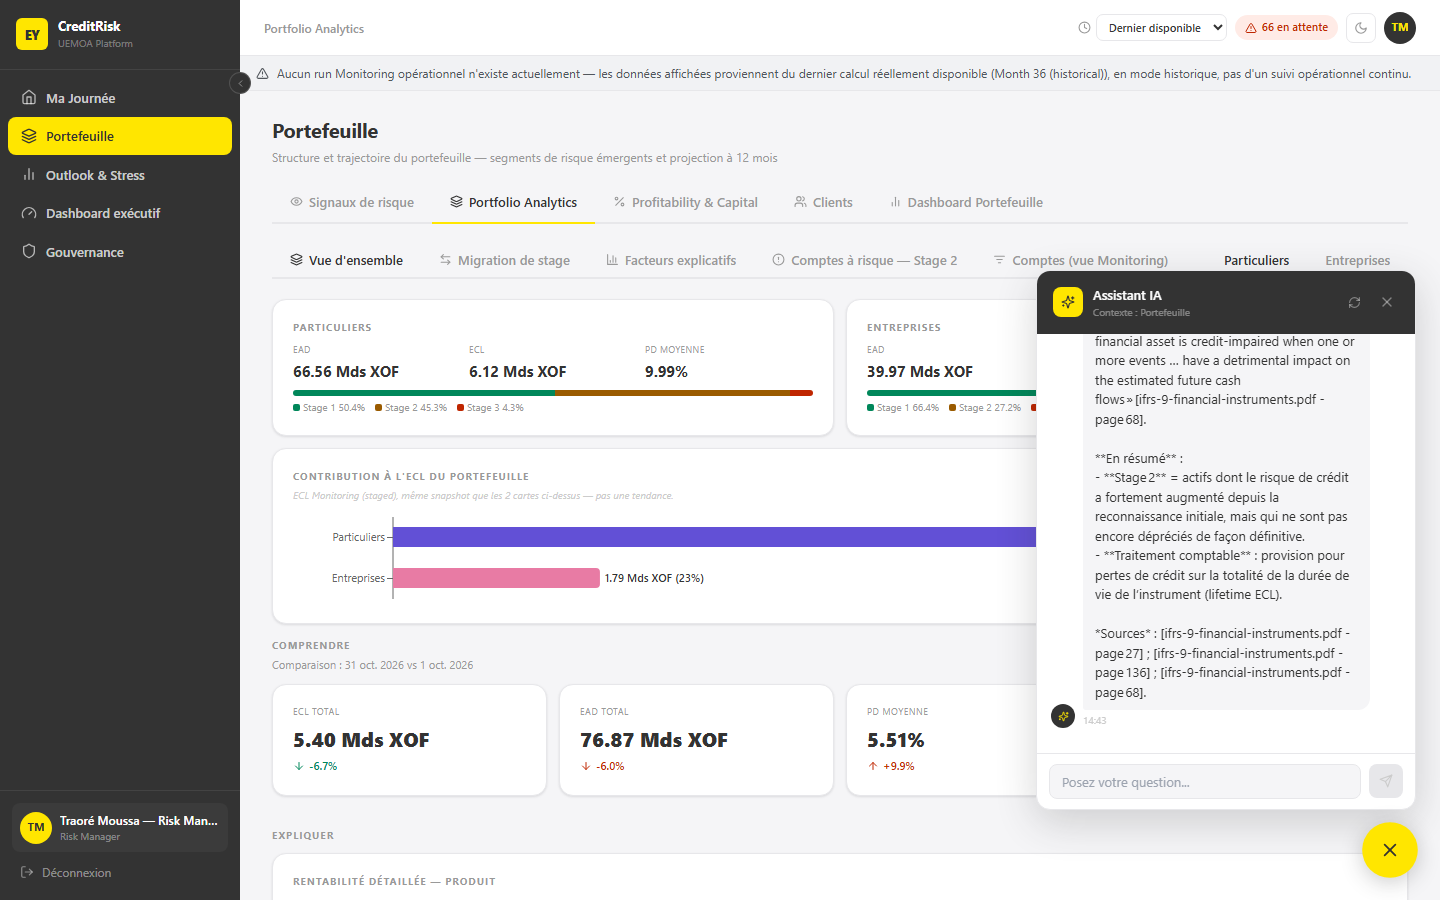
\includegraphics[width=0.85\textwidth]{figures/capture_assistant.png}
\caption{Assistant transversal — réponse appuyée sur la base documentaire réglementaire, avec citation de la source}
\label{fig:capture-assistant}
\end{figure}

\section{Tests et validation}

La stratégie de validation repose sur quatre marqueurs \texttt{pytest} réels, présentés en section~6.1, unitaire, intégration base de données, chaîne de traitement et acceptation, auxquels s'ajoutent, distincts de ce quatrième marqueur, deux scénarios d'acceptation en conditions de navigateur réel, exécutés séparément via Playwright. Les résultats présentés ci-dessous sont ceux d'une exécution réelle de l'ensemble de ces suites, et non des chiffres de référence : chaque échec rencontré a été rejoué isolément, et pour les plus significatifs directement inspecté dans ses artefacts (fichiers de données, journal d'audit), afin d'en caractériser la nature et, lorsque les éléments disponibles le permettent, d'en identifier la cause, plutôt que de les rapporter tels quels depuis un premier passage.

\subsection{Tests unitaires}

La suite unitaire, 351 tests collectés sur des composants isolés sans dépendance système réelle, s'exécute entièrement avec succès : 349 réussis, 2 ignorés, aucun échec.

\subsection{Tests d'intégration base de données}

La suite d'intégration, exécutée contre une instance PostgreSQL réelle, comporte 619 tests marqués, dont 614 réussis, 2 ignorés et 3 échecs, tous dans le même fichier (\texttt{test\_online\_data\_purity.py}). Ces trois échecs partagent une cause commune, confirmée en les rejouant isolément : trois assertions comparent le nombre de décisions en ligne authentiques à une valeur figée, 170, verrouillée au moment de la rédaction du contrat de test correspondant (2026-09-16), alors que la base contient désormais 449 décisions de ce type, un écart qui reflète l'usage réel de la plateforme accumulé depuis cette date plutôt qu'une régression. Le mécanisme d'exclusion lui-même reste par ailleurs démontré correct par ces mêmes échecs : les deux grandeurs comparées à la valeur figée, le décompte brut filtré et la vue \texttt{LIVE}, restent strictement égales entre elles (449 de part et d'autre), ce qui est précisément ce que le test cherche à vérifier au-delà du chiffre lui-même.

\subsection{Tests de chaîne de traitement}

La suite de pipeline, 341 tests marqués, totalise 334 réussis, 1 ignoré et 6 échecs. Cinq de ces six échecs relèvent de la même famille que les échecs d'intégration ci-dessus, une valeur ou un artefact figé devenu obsolète plutôt qu'une régression fonctionnelle : un test attend 60 lignes dans la dimension temporelle du Monitoring et en trouve 179, la couverture temporelle réelle s'étant élargie depuis l'écriture du test ; trois tests lisent un export Parquet des features Particuliers antérieur à l'ajout de certains champs aujourd'hui mobilisés par la plateforme (\texttt{revenu\_mensuel\_xof}, \texttt{stabilite\_profil}), confirmés par ailleurs omniprésents dans le code source actuel, du service de crédit en ligne au moteur d'explication ; un quatrième test, dépendant du même export, échoue en cascade faute de retrouver le premier identifiant client de ce fichier devenu obsolète dans l'état actuel de la plateforme. Le sixième échec est d'une nature différente : la validation d'un document dont le chemin de fichier n'existe pas renvoie \texttt{is\_valid=True} plutôt que \texttt{False}, le pipeline d'extraction ne consignant aucune erreur de validation pour un fichier absent avant le calcul de ce statut.

\subsection{Tests d'acceptation}

Le quatrième marqueur \texttt{pytest}, distinct des scénarios navigateur présentés plus loin, comporte 37 tests répartis sur plusieurs scénarios métier complets (création puis scoring d'un dossier réel, accord sous conditions jusqu'à leur résolution). 27 réussissent, 10 échouent, répartis en deux anomalies réelles et distinctes, toutes deux rejouées et inspectées directement pour en établir la cause.

La première touche neuf tests, répartis sur deux fichiers de scénario dont l'un des paramètres de la demande (profil \emph{Fonctionnaire}, garantie de type caution, ratio de couverture à 1,00) est quasiment identique : dans le premier fichier, un dossier réellement créé et scoré au cours de ce passage présente une exposition, une PD et un hurdle rate persistés à zéro, trois assertions qui en dépendent échouant en conséquence ; dans le second, c'est l'étape initiale du scénario qui échoue directement, sur une erreur Python (\texttt{TypeError}, valeur \texttt{None} inattendue), les cinq étapes suivantes échouant alors en cascade faute de retrouver l'état qu'elles présupposent. Ces deux échecs partagent un profil de demande très proche et pourraient relever d'une même cause, sans que cette campagne de validation permette de l'affirmer avec certitude : l'établir précisément dépasserait le cadre de cette synthèse et relèverait d'une correction à part entière.

La seconde anomalie, isolée, porte sur l'intégrité du journal d'audit chaîné présenté au chapitre 2 : \texttt{verify\_integrity()} détecte une rupture de la chaîne de hachage. L'inspection directe du fichier concerné situe précisément cette rupture : deux entrées \texttt{DATA\_ACCESS} de l'assistant, consécutives, portent un horodatage strictement identique à la microseconde (deux questions quasiment identiques posées le 2026-09-29) et référencent toutes deux le hachage de l'entrée qui les précède, au lieu que la seconde référence le hachage de la première. Il s'agit d'une véritable condition de concurrence sur l'écriture de ce journal en cas d'appels strictement simultanés, antérieure à cette campagne de validation, et non d'une altération a posteriori du journal ni d'un artefact introduit par l'exécution des tests eux-mêmes.

\subsection{Tests d'acceptation en conditions de navigateur}

Les deux scénarios Playwright, séparés du quatrième marqueur \texttt{pytest} ci-dessus, couvrent chacun un parcours bout en bout complet, en conditions de navigateur réel : Origination (client existant jusqu'au Cas Crédit, en passant par la création du dossier et le scoring) et Surveillance (cycle réel de Monitoring jusqu'au Cas Crédit existant). Le scénario Origination réussit intégralement. Le scénario Surveillance échoue à son script de préparation, avant même d'atteindre l'interface : le compte sélectionné pour ce scénario ne déclenche plus de trigger de dégradation dans l'état actuel de la base, la même famille d'anomalie que celle déjà rencontrée pour les tests d'intégration et de pipeline, un scénario de test ancré sur un état précis d'une base de données réelle qui continue d'évoluer.

\subsection{Synthèse}

Sur l'ensemble des suites \texttt{pytest} et des deux scénarios Playwright, 1\,325 tests ou scénarios réussissent sur 1\,345 exécutés, hors tests ignorés, soit 20 échecs. Neuf relèvent d'une valeur ou d'un artefact de test figé à une date donnée, devenu incohérent avec l'état réel, aujourd'hui plus avancé, d'une base de données et d'une plateforme en usage continu, plutôt que d'un défaut des composants testés. Les onze autres correspondent à trois anomalies réelles et distinctes : un pipeline d'extraction documentaire qui ne signale pas l'absence d'un fichier, un scénario de demande à un profil de garantie particulier qui produit une exposition, une PD et un hurdle rate nuls ou une erreur selon le point d'entrée, et une rupture ponctuelle, mais réelle et précisément datée, de la chaîne de hachage du journal d'audit lors de deux écritures strictement simultanées.

Cette synthèse ne doit pas être confondue avec une validation complète de l'exactitude métier de la plateforme, qui dépend aussi des hypothèses de modélisation déjà discutées aux chapitres 3 et 4, ni masquer deux limites distinctes des suites de test elles-mêmes : leur robustesse face à l'évolution continue des données qu'elles interrogent, déjà discutée pour les neuf échecs liés à l'obsolescence des données et artefacts de test, et la profondeur de diagnostic qu'elles permettent au-delà du constat d'échec, les causes exactes des neuf échecs répartis entre les deux scénarios de demande, ainsi que l'existence éventuelle d'une cause commune, restant à isoler précisément par une investigation dédiée, hors du cadre de cette campagne de validation.

\section{Bilan de réalisation}

\subsection{Résultats obtenus}

La plateforme réalisée intègre effectivement les composantes fonctionnelles et transversales annoncées en introduction de ce rapport, et non une juxtaposition de démonstrateurs isolés : un parcours d'Origination en temps réel et un traitement Portfolio Analytics par batch, qui s'appuient sur des composants de calcul de risque de même nature tout en conservant leurs propres artefacts de modèles et leurs logiques de traitement distinctes, le batch mobilisant une politique de recommandation dédiée (\texttt{DecisionSupportPolicy}) plutôt que le moteur de décision complet d'Origination ; un contrôle d'accès par rôle appliqué côté backend, à chaque point d'entrée de l'API plutôt qu'à la seule interface ; une gouvernance et une traçabilité alimentées par les exécutions réelles de la plateforme, et non par un mécanisme déclaratif ; enfin, un assistant conversationnel qui interroge ces mêmes composants sans recalculer les indicateurs de risque ni se substituer au moteur de décision. Cette intégration est illustrée par les captures d'écran de la section~6.4, prises sur l'application réellement exécutée, et étayée par la campagne de validation présentée en section~6.5, au cours de laquelle 1\,325 tests et scénarios automatisés ont réussi sur 1\,345 exécutés. Les échecs restants, analysés et caractérisés, permettent également de préciser les limites actuelles de l'implémentation.

\subsection{Difficultés rencontrées et ajustements}

Plusieurs difficultés concrètes ont marqué cette phase de réalisation et de validation, distinctes des choix de conception déjà discutés au chapitre 5. Le démarrage du backend a d'abord révélé un défaut d'encodage de console sous Windows, sans lien avec la logique applicative, diagnostiqué et corrigé ligne par ligne plutôt que supposé. La rédaction de la section~6.2 a par ailleurs mis en évidence que la description des traitements Origination et Portfolio Analytics glissait, par endroits, vers une description déjà donnée par les diagrammes de conception du chapitre 5 : la distinction retenue, un renvoi à ces diagrammes plutôt qu'une répétition de leur contenu, complétée par quelques ancrages courts sur le déroulement réel, a dû être ajustée au fil de la rédaction. La construction de la section~6.3 a de même révélé que deux diagrammes structurants du rapport, le diagramme de cas d'utilisation du chapitre 2 et le diagramme de classes du chapitre 5, avaient été établis avant que l'assistant ne soit traité en profondeur et ne le représentaient donc pas, une omission corrigée a posteriori plutôt que découverte dès l'origine. Enfin, la campagne de validation de la section~6.5 a nécessité d'élargir les vérifications au quatrième marqueur \texttt{pytest}, consacré aux scénarios d'acceptation, puis de distinguer, parmi les échecs obtenus, ceux dus à des données de test devenues obsolètes de ceux relevant d'anomalies fonctionnelles réelles. Ce travail de diagnostic a notamment permis de retracer une rupture de la chaîne d'audit jusqu'à deux écritures strictement simultanées.

\subsection{Limites restantes}

Les limites identifiées au cours de cette phase se distinguent de celles, méthodologiques, déjà posées aux chapitres 3 et 4 : l'échantillon Corporate restreint pour le modèle de LGD, l'absence de preuve de généralisation hors échantillon pour la sélection par BIC, ou la disjonction entre capital proxy et capital Monte Carlo jamais combinés dans le RAROC. La campagne de validation de la section~6.5 ajoute trois limites propres à l'implémentation, non corrigées à ce stade : un pipeline d'extraction documentaire qui ne signale pas explicitement l'absence d'un fichier, un scénario de demande à un profil de garantie particulier qui produit des indicateurs financiers nuls ou une erreur selon le point d'entrée emprunté, et une fenêtre de concurrence, ponctuelle mais réelle, dans l'écriture du journal d'audit lors d'accès strictement simultanés. À ces limites s'ajoutent celles, plus larges, déjà posées par la nature du projet : les données exploitées restent synthétiques, et la plateforme n'a été ni déployée ni exploitée en environnement de production. Le volume de tests réussis présenté en section~6.5 apporte ainsi des éléments de validation du fonctionnement logiciel de la plateforme, pas de la validité prédictive de ses modèles ni de sa conformité à un cadre réglementaire, deux questions distinctes, déjà traitées pour ce qu'elles permettent réellement d'affirmer aux chapitres 3 et 4.

\section*{Conclusion du chapitre}

Ce chapitre a montré comment l'architecture présentée au chapitre 5 a été effectivement construite, puis mise à l'épreuve. L'environnement technique mobilise des technologies choisies pour un usage précis plutôt que juxtaposées ; les parcours d'Origination et de Portfolio Analytics s'appuient sur des composants de calcul communs tout en conservant leurs logiques propres, et sont complétés par des mécanismes transversaux d'authentification et de gouvernance ; l'assistant conversationnel, construit sur ce même socle, reste strictement circonscrit à son rôle de lecture, sans jamais recalculer ni décider ; et les interfaces, parcourues écran après écran selon l'arborescence réellement implémentée, donnent à voir cette réalisation du point de vue de l'utilisateur. La campagne de validation qui referme ce chapitre a confronté l'ensemble de ces réalisations à des exécutions effectives de la plateforme, plutôt qu'à une liste de fonctionnalités supposées correctes, et le bilan qui en découle distingue ce qui a été obtenu de ce qui reste, à ce stade, une limite assumée. C'est sur cette base, celle d'une plateforme réellement construite et dont les limites sont connues plutôt que supposées absentes, que se referme ce rapport, dont la conclusion générale revient sur l'ensemble du travail mené depuis la construction des modèles jusqu'à cette réalisation.
